%{{{ Spam
\documentclass[a4paper,12pt]{article}

%use danish hyphenation and titles
%handle utf8-characters
\usepackage[danish]{babel}
\usepackage[utf8]{inputenc}
\usepackage[T1]{fontenc}

%for images
\usepackage[pdftex]{graphicx}

%allow nested figures
\usepackage{subfigure}

%control line spacing
\usepackage{setspace}
%\singlespacing
\onehalfspacing
%\doublespacing

%set margins
%\usepackage[margin=0.75in]{geometry}

%allows margin-notes
%good for work in progress papers
%\usepackage{marginnote}

%allows pretty quoting using ``'' or `'
\usepackage{upquote}

%two definitions of the color grey
\usepackage{color}
\definecolor{listinggray}{gray}{0.9}
%\definecolor{lbcolor}{rgb}{0.9,0.9,0.9}


% References
\usepackage{hyperref}

%allows pretty source code
\usepackage{listings}
\lstset{
  language=,
  literate=
    {æ}{{\ae}}1
    {ø}{{\o}}1
    {å}{{\aa}}1
    {Æ}{{\AE}}1
    {Ø}{{\O}}1
    {Å}{{\AA}}1,
  backgroundcolor=\color{listinggray},
  tabsize=3,
  rulecolor=,
  basicstyle=\scriptsize,
  upquote=true,
  aboveskip={1.5\baselineskip},
  columns=fixed,
  showstringspaces=false,
  extendedchars=true,
  breaklines=true,
  prebreak =\raisebox{0ex}[0ex][0ex]{\ensuremath{\hookleftarrow}},
  frame=single,
  showtabs=false,
  showspaces=false,
  showstringspaces=false,
  identifierstyle=\ttfamily,
  keywordstyle=\color[rgb]{0,0,1},
  commentstyle=\color[rgb]{0.133,0.545,0.133},
  stringstyle=\color[rgb]{0.627,0.126,0.941},
}
%captions on listings
\usepackage[center,font=small,labelfont=bf,textfont=it]{caption}

%allows fancy enumeration
\usepackage{enumerate}

%allows use of the BibTex for the bibliography
\usepackage[numbers]{natbib}

%make references and URLs in the pdf to clickable links
\usepackage{hyperref}

%removes the numbers from sections
\setcounter{secnumdepth}{0}


%proper header formatting
\usepackage{fancyhdr}
\pagestyle{fancy}


%Rydder fancyheads(sidehoved) underlige tekst
\fancyhf{}
\lhead[]{} %clear standard settings
\chead[]{} %clear standard settings
\rhead[]{} %current section
\lfoot[]{} %clear standard settings
\cfoot[]{\thepage} %current page number 
\rfoot[]{} %clear standard settings
\usepackage{float}
\usepackage{hyperref} % The package for links. This is also used for the ToC links.


\title{Heartbeat protokollen \\ Bachelorprojekt 2015}
\author{Erik Allin - smt504 \\ Dennis Olesen - cwb579}
\date{8. juni 2015}

%Centreret sidehoved
\chead{Erik Allin - smt504 \& Dennis Olesen - cwb579}

\begin{document}
\maketitle
\newpage
\renewcommand*\contentsname{Indholdsfortegnelse}
\tableofcontents
%\section*{Forside-lel}
\newpage
\clearpage

\section{Resumé}
Vi undersøger muligheden for, at kunne implementere et Heartbeat-bibliotek til eksempelvis load-balancing af servere, med et simpelt brugerinterface. Dette giver brugeren et delt dictionary som fælles data samt overblik over liveliness af samtlige systemer.
\\
Som konsensus implementeres Raft-algoritmen, som udfører leader-election på ned til 300-400 ms uden forkerte valg. 

\section{Abstract}
We explore the opportunity of implementing a Heartbeat-library for solving such issues as load-balancing of servers with a simple user interface. This gives the user a shared dictionary as shared memory along with an overview of liveliness of all related systems.
\\
Using the Raft-algorithm for consensus, which applies leader-election in about 300-400 ms without any errors.
\newpage

\section{Beskrivelse af problemet}
I forbindelse med udvikling af et distribueret system vil man være afhængig af, at kunne sikre sig konsistens samt høj tilgængelighed af det involverede system samt at systemet er tolerant over for partitioneringer. Metoder til at opdage når en maskine fejler, samt derefter at foretage de nødvendige fejlprocedurer, vil altså være at finde i størstedelen af de distribuerede systemer.
\\
Ved at konstruere et bibliotek, som gør det simpelt for brugeren at implementere disse metoder, vil der både kunne spares udviklingstid for fremtidige projekter, der omhandler distribuerede systemer. Derudover vil det være et fælles produkt at kunne optimere og opdatere, fremfor at skulle tage hensyn til hvert enkelt nyudviklede system. 
\\[5px]
Der kan eksempelvis ses på en case, hvor der skal håndteres en række servere stående lokalt hos en mindre virksomhed. Denne virksomhed ønsker, at lave en simpel håndtering af hvilke maskiner der er aktive samt en håndtering af ressourcestyringen for hver af maskinerne. Denne ressourcestyring gør så den maskine med lavest belastning altid får den næste opgave. For at gøre dette ønskes der lavet et bibliotek, der tillader maskinerne at snakke sammen regelmæssigt og derved have mest mulig tid, hvor systemet er tilgængeligt. Dette ønskes at kunne blive implementeret så simpelt som muligt, da systemet skal implementeres uden at nogle i virksomheden har nogen forudgående forståelse for hvordan systemet fungerer.
\\[5px]
Et sådant bibliotek vil altså kunne sikre fremtidige applikationer, der bruger distribuerede systemer, en fælles og gennemtestet implementation til overvågning af aktive og inaktive systemer, samt en fælles hukommelse så maskinerne kan tale med hinanden alt efter af brugerens behov.

\subsection{Redegørelse}
For at kunne lave et bibliotek til implementering af eks. ressourcestyring via heartbeat protokollen, så er vi nødt til, at forstå hvordan systemet skal hænge sammen.
\\
I et sådant system er det meget relevant, hvordan dataen der kommunikeres mellem de forskellige maskiner i systemet, bliver sendt rundt el. håndteret.
Der findes forskellige modeller, for hvordan dette kan gøres, hvor den simpleste er, at alle maskiner kommunikerer med alle.
Derved sørges der for, at alt data kommunikeres rundt blandt alle maskiner, så på dette område, ville dette system være tilstrækkeligt. 
Det kan dog godt hurtigt gå hen og blive meget ressourcekrævende, da vi opnår $n^2$ antal forbindelser, da alle maskiner skal kommunikere med alle de andre.
\\[5px]
Dette kan reduceres kraftigt ved at benytte gossiping [4], hvor en maskine skriver ud til en vilkårlig anden maskine, som herefter skriver ud til nogle andre, og så videre indtil beskeden er propageret ud til samtlige maskiner i systemet.
\\
Her vinder man dog mest i meget store systemer, hvor det ikke kan lade sig gøre at fordele en besked rundt alle maskiner samtidig.
\\[5px]
En lidt anderledes tilgang er at have en leder, der styrer alt kommunikation, samt at resten af maskinerne er følgere, der lytter på lederen og svarer tilbage når de modtager et heartbeat. Dette sikrer at alle følger-maskinerne kun skal sende en besked, mens at lederen derimod sender ud til alle følgerne. Dette vil give os, at lederen skal sende lige så mange beskeder, som der er af følgere, mens følgerne kun sender en hver. 
Dette giver os en væsentlig forbedring i antal beskeder end eksempelvist hvis alle snakker med alle. Dette har imidlertid det problem at der vil være en single-point-of-failure i forbindelse med lederen, da systemet ikke kan køre uden lederen. For at undgå dette kan man vælge en protokol for at vælge en ny leder, i tilfælde af at den forrige mister forbindelsen. 
\\[5px]
En simpel måde at gøre dette er via Bully algoritmen [5] hvori, at hver maskine får tildelt et ID, og såfremt lederen dør, så vælges den leder med det højeste ID. Dette kan lade sig gøre ved, at lade hver maskine sende en besked til alle maskiner med højere ID end sin egen, og såfremt den ikke modtager et svar tilbage lader den sig selv blive leder. Dette er en relativ simpel algoritme, der dog ikke tager hensyn til problemer ved partitionering, da man kan risikerer, at der kan opstå flere systemer samtidig. 
\\[5px]
Dette problem kan løses ved at bruge algoritmen som bruges i Raft [3], der bruger et system bestående af følgere, kandidater og leder.
Når en leder undervejs går hen og dør, starter der et leader-election, hvor der vælges den hurtigste kandidat, som har mindst halvdelen af stemmerne, til at blive leder. Herved sikres det, at der kun vælges en leder, og derved risikerer vi ikke i stil med Bully algoritmen, at der kan opstå flere systemer parallelt med hinanden.
\newpage
  
\section{Problemorienteret analyse}
I stil med Raft \textbf{[3]} skal vi have en leder, der kan uddelegere opgaver, samt overvåge aktiviteten (liveliness) for de resterende systemer. Dette kan lederen gøre ved regelmæssigt at sende heartbeats ud til alle de aktive følgere. I forbindelse med dette tjek af liveliness, kan brugeren sende en værdi for evt. belastningen med vores heartbeats, der sendes til følgerne. Dette tillader brugeren, at lave en prioritering for hvilke følgere, der skal modtage næste opgave.
\\
Da vi er interesserede i, at systemet også skal have høj tilgængelighed er vi afhængige af at lederen ikke er en single-point-of-failure. Kort sagt må systemet ikke fejle når en vilkårlig maskine fejler.
\\[5px]
Dette kan vi undgå ved, at have mulighed for at vælge en ny leder, når følgere i en længere periode ikke har modtaget heartbeats fra lederen. Dette gøres i stil med Rafts leader-election \textbf{[3]}, hvor de fjernes ved omkring 3 på hinanden følgende udeblivelser. Heri anvendes der kandidater, som følgere kan skifte status til, hvis de ikke modtager heartbeats i en længere periode, ca. 3 heartbeats, fra lederen. Herudover er det målet, at kandidaterne så vidt som muligt er up-to-date og har en delt tilstand. 
\\
Loggen er en metode, som vi bruger til at dele information om hvilke maskiner der er aktive, samt brugerdefinerede data uden at skulle sende hele informationen hver gang. Dette sparer ressourcer og sikrer at alle parter har den samme information.
\\[5px]
Dette system vil altså afhænge af, at have fem del-funktionaliteter der tilsammen udgør systemet. Disse fem funktionaliteter kan ses som Discovery, hvor der oprettes forbindelse til følgere på netværket, hvilket også vil blive beskrevet nærmere senere. Derudover er der liveliness hvor der regelmæssigt tjekkes for, at følgere og leder er i live. Leader-election sikrer, at der hurtigt kan findes en ny leder, hvis den nuværende fejler. Logging sikrer sig, at der hele tiden er en vis konsistens i systemet, så alle medlemmer i systemet har den samme information, eller hurtigst muligt retter op og når en committed state, når der vælges en ny leder. Til sidst er der load-balancing, som afhænger af at det resterende system fungerer, så det kan balancere belastningen af følgerne på applikationsniveauet i forhold til vores case eksempel.

\subsection{Beskrivelse af konsistensmodeller}
I forbindelse med at der arbejdes på distribuerede systemer vil det være nødvendigt at have en konsistens model. Dette sikrer, at vi kan have en fælles state på alle maskiner. 
Der findes dog en lang række konsistens modeller, og det er derfor nødvendigt, at finde den rette til vores formål. En række af disse modeller, er dem som er beskrevet herunder. \textbf{[8]}
\\[5px]
\textbf{Strict Consistency}
\\
Strict consistency modellen er som det meget ligger i navnet den optimale model, idet den sikrer til enhver tid, at alle der læser fra et pågældende system vil læse den seneste besked, der er skrevet til systemet. Derudover vil den besked der skrives først, altid være først i rækkefølgen. Dette er imidlertid ikke muligt, at opretholde såfremt man arbejder på mere end en kerne, da to samtidige skrive-operationer vil kunne ødelægge denne model, da der opstår uenighed om hvilken skrive-operation, der er udført først.
\\[5px]
\textbf{Sequential Consistency}
\\
Vil vi den forrige models problem til livs, kan det være værd at se på sequential consistency modellen. Heri er rækkefølgen på skrevne operationer afhængigt af hvornår der er enighed om, at denne operation er udført. Dette er forskelligt fra strict consistency, da denne kræver at rækkefølgen er den samme som rækkefølgen af hvornår ting er blevet eksekveret.
\\[5px]
\textbf{Causal Consistency}
\\
Rykker vi ned og bliver endnu mindre strikse end i sequential consistency modellen, så kan vi se på causal consistency. Heri kan writes, der ikke er kausalt afhængige af hinanden godt ses i forskellig rækkefølge på forskellige maskiner. Der gælder dog, at hvis de er kausalt afhængige, så skal rækkefølgen opretholdes - en write, \textit{write2} der er kausalt afhængig af en tidligere write, \textit{write1} må altså vente til, at \textit{write1} er tilføjet det samlede system før den selv kan blive det.
\newpage

\section{Programmerings overvejelser}
\subsection{Discovery}
For at skabe forbindelse til maskiner på et lokalt netværk, er man, som vi kom frem til i forrige afsnit, nødt til at benytte sig af en Discovery protokol. Et sådant system kendes også som Network Discovery services, som set i DSCD \textbf{[6]}. Normen er her, at man opretter forbindelse til andre systemer i netværket, ved at broadcaste eller multicaste. \textbf{[7]} Derved kan man få beskeden ud til de resterende systemer. Broadcast virker som den oplagte måde, at gøre det på da der arbejdes på et lokalt netværk.
Ville man ændre modulet til at fungere på internettet, frem for på det lokale netværk, kunne multicast med fordel anvendes.
Problematikken er i midlertidig om det er en directory server eller serverless model, der vil fungere bedst i forbindelse med resten af systemet.
\\[5px]
Her kan man argumentere for, at en directory server ville give mening, da der i forvejen sendes regelmæssige broadcasts i forbindelse med heartbeat. Altså kunne man her bruge heartbeatet, som en forespørgelse til systemer, der ikke er forbundet med lederen endnu.
\\
Directory serveren har dog det problem, at hvis den går ned, er der ikke længere styr på hvilke maskiner, der er i systemet. Dette er imidlertid en problematik, som bør kunne løses ved at bruge en serverless metode med leader-election og logging, ved at man vedligeholder en replikeret log, som indeholder de aktive maskiner, til alle medlemmer i systemet. 
\\
Derved vil en ny leder have samme information, som den tidligere leder, såfremt man i stil med Raft-algoritmen ikke vælger en maskine der ikke er up-to-date, og kan derved overtage jobbet uden at miste konsistens eller tilgængelighed, da der kun afgives stemmer til kandidater der har en opdateret log. Ifølge DSCD [6], bruges der leasing til, at sikre sig, at maskinerne er aktive. Dette må kunne opretholdes med heartbeats, da dette foretager samme tjek, altså ved feedback om et kald, el. en service går igennem.

\subsection{Broadcast/MultiCast/UDP/TCP}
Selve valget om hvorvidt man skal bruge broadcast eller multicast er ikke helt trivielt da de begge har fordele og ulemper der påvirker systemet. Forskellene ligger i at broadcast arbejder med UDP forbindelse mens, at multicast bruger TCP \textbf{[7]}.
\\
Fordelen ved broadcast og UDP forbindelser er, at vi sparer ressourcerne det kræves at skabe en fast forbindelse med hver enkelt følger i systemet. Vi kan endvidere, såfremt vi forbliver lokalt, udnytte broadcast til at kommunikere heartbeats ud til alle medlemmer i systemet, hvilket er den billigste måde at kommunikere med alle på en gang. Endvidere tillader dette os, at tilføje nye maskiner løbende ved at klienten hører det broadcastede heartbeat og sender svar til lederen, uden at skulle kende lederens IP-adresse på forhånd, hvor man i tilfældet med multicast ville være afhængig af at en følger skulle kende lederen på forhånd. Derudover fungerer heartbeats på den måde at det ikke gør nogen reel skade hvis der misses en besked eller to, da det næste kommer kort efter. Dette betyder selvfølgelig at der vil være en længere periode mellem konsistens, men ikke noget der er meget langsommere end at lave og afslutte TCP forbindelser til alle modtagere.
Herudover er både UDP og TCP implementeringer af systemet begrænset ved skalering.
\\[5px]
UDP har oftest loft over pakkestørrelse der giver problemer når loggens størrelse nærmer sig de ca. 1500 bytes \textbf{[2]}. Dette er grundet, at der på link-laget som regel sættes et MTU, Maximum Transmission Unit, for bedre at fungere med den reelle buffer størrelse. TCP er derimod begrænset af hastigheden da multicast bliver tungt i forbindelse med oprettelse af forbindelse til mange systemer ad gangen. 
I vores implementation benyttes broadcasting, da modulet er tiltænkt lokale systemer.
Dette betyder endvidere at den største begrænsning for køretid og effektivitet er relateret til hardwaremæssigt at sende beskeder på tværs af maskiner.

\subsection{Liveliness} 
Liveliness er langt hen ad vejen en af grundidéerne ved heartbeat. Derfor ligger det også naturligt, at liveliness bliver tjekket via heartbeats, samt manglen heraf. Man kan definere et system til, at være i live, når det har forbindelse til lederen. Ved brug af leader-election, som ses senere vil der altid være en ny leder, der kan erstatte en afgående, el. død leder (inden for et rimelig interval). I praksis vil tjek for liveliness ligge meget op ad det, der er omtalt i Discovery-afsnittet.
\\
Dette grundet at heartbeats er måden hvorpå liveliness tjekkes, og at listen over aktive, el. levende, systemer opbevares i en log, som bliver opdateret løbende igennem Discovery-protokollen samt via brugerinput.

\subsection{CAP-teoremet og dets begrænsning af systemet}
CAP teoremet er idéen om at et distribueret system ikke kan vedligeholde de tre følgende kvaliteter på en gang: Konsistens, tilgængelighed og partitions-tolerance. Ifølge CAP er det kun muligt at have to af disse ad gangen. Dette betyder i vores tilfælde hvor vi ønsker høj tilgængelighed samt tolerance over for partitionering, at vi ikke kan forvente at have konsistens i alle tilfælde hvor systemet partitionerer.
Den høje tilgængelighed eksistere i form af at der altid vil være en aktiv leder, da en ny vælges umiddelbart efter mistet forbindelse med den gamle.
\\
Dog kan dette fejle såfremt der sker en for stor partitionering af systemet. 
I Raft [3] fungerer leader-election ved at man kun kan blive leder såfremt man har over halvdelen af stemmerne, for at sikre at der ikke eksisterer to samtidige uafhængige systemer. Dette betyder til gengæld at hvis halvdelen af systemerne plus lederen, eller flere, falder fra samtidig, vil de tilbageværende følgere ikke kunne blive ledere, da de antager at de skal have n/2 stemmer men der kun er højst (n/2)-1 systemer tilbage. 

\subsection{Leader-election} 
Da vi ønsker at opbygge vores system i stil med Raft-algoritmen, er leader-election en essentiel del af dette heartbeat system. Det sørger for at såfremt lederen, altså det system der modtager og videresender forespørgsler, skulle stoppe med at fungere, så vil der, under enighed mellem alle i systemet, blive valgt en ny leder.
\\
For at gøre dette, kan man, i stil med Raft [3], indføre tre stadier for systemerne:
\\
Følger, kandidat og leder.
\\[5px]
Disse fungerer ved, at ved at en følger kan blive kandidat, såfremt den ikke har modtaget beskeder fra lederen i en tidsbestemt periode. Når en følger bliver kandidat udsteder den et valg, og sender en forespørgsel om at blive valgt som en ny leder. Såfremt kandidaten får majoriteten af stemmerne, vil den blive valgt som den nye leder.
\\
Lederens rolle er at lytte på klienten som sender forespørgsler, og så sørge for at disse forespørgsler bliver sendt ud til de korrekte systemer, samt sikre sig konsistens i loggen.
\\
For at undgå at systemer der ikke er up-to-date kan være ledere, er der indført en logisk klokke til at holde styr på at alle systemer er lige langt. 
Dette sikrer at hvis en maskine kommer ud af synkronisering vil den ikke kunne blive leder, samt at hvis en leder mister forbindelsen og der bliver valgt en ny leder, vil den når den kommer tilbage opdage at den ikke længere skal være leder, og derved skifte til følger.
\\
\begin{figure}[H]
  \caption{Raft leader-election.}
  \centering
    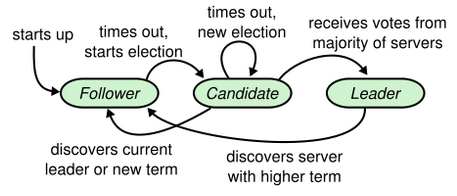
\includegraphics[width=0.8\textwidth]{Raftleaderelection.png}
\end{figure}


\subsection{Logging}
For at systemet hele tiden kan holdes konsistent, må vi indføre en form for logging. Logging sørger for, at alle medlemmer af systemet hele tiden kan holde styr på, om de er med i systemet. Samtidig sikrer loggen en trinvis opdatering af den delte tilstand. Hvis de f.eks. mister forbindelsen i en periode, og så kommer tilbage i systemet, så vil medlemmet højst sandsynligt være kommet bagud i forhold til resten af systemet, og derved skal medlemmet ikke f.eks. forsøge at blive kandidat, der vil kunne forsinke systemet (som også beskrevet i forrige afsnit). 
\\
Loggingen laves via timestamps og en logisk klokke, så der hele tiden kan ses hvilket stadie de forskellige dele af systemet er nået til. Derudover holder loggingen også styr på rækkefølgen det hele skal foregå i, for derved at kunne se, hvis nogle opgaver ikke er blevet udført af de forskellige dele af systemet. Dette sikres ved, at loggen hele tiden holdes konsistent og hele tiden bliver replikeret ud til alle medlemmer af systemet. Derved sikres det også, at når en ny leder bliver valgt, så vil denne leder også have den log, som den forrige leder havde, og derved går der ikke nogle opgaver tabt.
\\[5px]
Når loggen skal replikeres ud til følgerne er det en fordel for skaleringen at sende opdateringer til systemernes log frem for at gensende hele loggen hver gang.
Dette kan man gøre ved at sende opdateringer som (key, data) par, hvor key repræsenterer en logisk klokke der sikre at de bliver tilføjet i konsistent rækkefølge, og dataen er en funktions-repræsentation der fortæller loggen hvad den skal opdatere.
\\
Her vil det dog stadig være nødvendigt at sende hele loggen når et nyt system tilslutter sig. Endvidere kan det betale sig at committe når alle deltagere i systemet har den samme log, da vi herved kan undgå at loggen skalere i forhold til tiden systemet har kørt. Dette vil forhindre hukommelsesproblemer i det længere løb.


\subsection{Load-balancing}
I forbindelse med casen nævnt i afsnittet om motivation, er brugeren interesseret i at implementere et program til at håndtere belastningen af de forskellige servere. Dette kan heartbeat systemet tillade ved at lade brugeren opdatere en bruger-log, hvor den enkelte maskine kan sende information, der bliver delt ud til resten af maskinerne via et Heartbeat. Som det ses af figur 2 vil et sådant system være bygget op således at en load balancer maskine holder styr på alle maskinernes load, når router(ne) så vil sende en opgave videre spørger den load-balanceren hvilke maskiner er klar, hvorefter den sender opgaven videre til den konkrete maskine.
Herefter svarer maskinen tilbage og load-balanceren modtager en opdateret værdi for maskinens belastning.

\begin{figure}[H]
  \caption{Load balancing.}
  \centering
    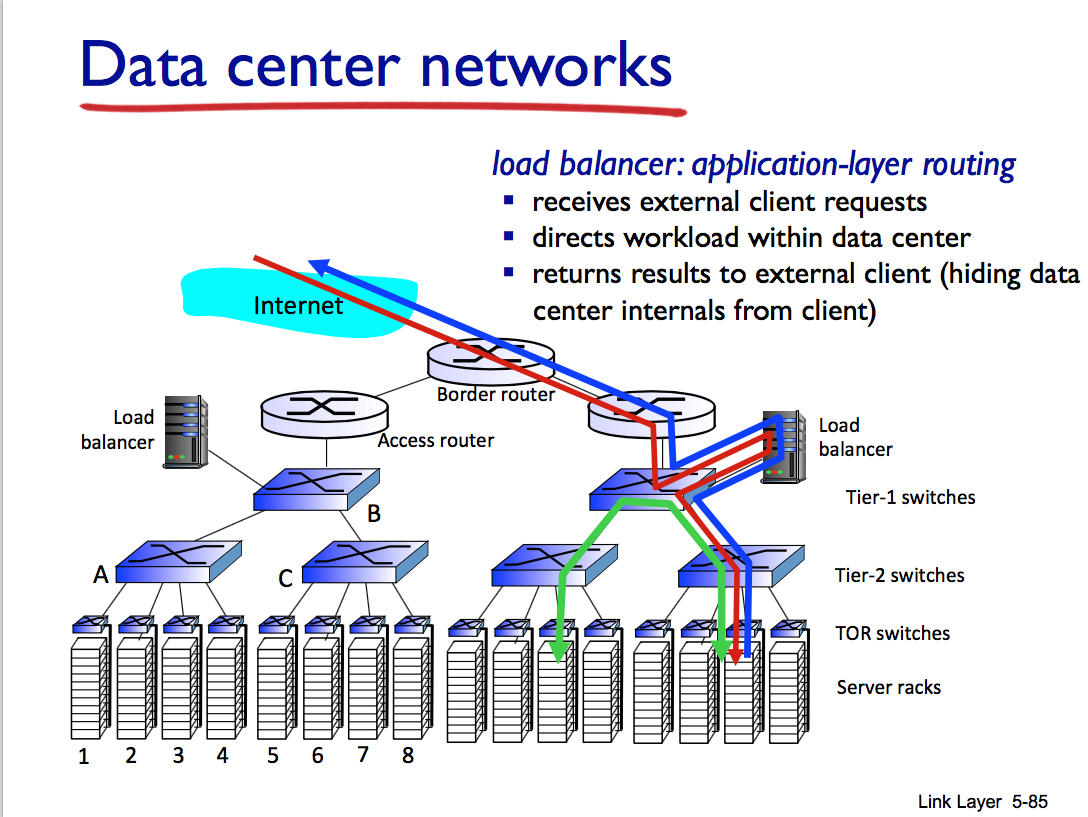
\includegraphics[width=1\textwidth]{Loadbalancing}
\end{figure}

\subsection{Valg af konsistensmodel}
For at sikre, at der vil være enighed omkring loggen samt bruger-opdateringer, på tværs af systemerne, så er vi afhængige af, at have valgt en konsistens model, der opfylder, at alle maskiner vil have de samme beskeder i samme rækkefølge.
\\[5px]
Hvis vi ser tilbage på de førnævnte tre konsistens modeller \textbf{[8]} i vores problemorienterede analyse, så kan vi ud fra disse vurdere, hvilken vi har gjort brug af.
Ser vi på strict consistency modellen, så må det hurtigt vurderes, at i vores system er det ikke tilfældet, at to samtidige skrive-operationer vil kunne ødelægge vores system, eller at den der skriver først nødvendigvis er den kommer først i rækkefølgen. I vores tilfælde er det lederen, der tildeler den pågældende operation en key, der så bestemmer rækkefølgen på operationerne.
Altså er strict consistency ikke den model, vi gør brug af.
\\[5px]
Kigger vi lidt på den modsatte side i forhold til hvor striks en model er, så ser vi på causal consistency. Heri gælder der specielle regler for, hvis operationer er kausalt afhængige. Sådanne regler benytter vi os ikke af vi vores system, da udførte operationer som sådan ikke har nogen indbyrdes afhængighed. I vores model er det blot den rækkefølge lederen modtager, og udsender udførte operationer, der bestemmer rækkefølgen, der er på tværs af systemet.
Endvidere gælder det for causal at kommandoer der ikke er kausale ikke behøves være samme rækkefølge på alle maskinerne, dette er ikke tilfældet i vores system, da alle skal have samme state.
\\[5px]
Vi kan endelig komme frem til, at vi i højere grad benytter os af sequential consistency modellen. Rækkefølgen på en skreven operation er afhængig af hvornår, der er enighed om denne i systemet. I vores tilfælde bestemmer lederen rækkefølgen, og sender den derefter ud til de andre systemer.

\subsection{Opsamling}
Vi vil altså implementere systemet via UDP beskeder, ud fra samme algoritme som er beskrevet i Rafts algoritme. Til dette vil vi dog gøre brug af en enkelt logisk klokke til håndtering af konsistentet, fremfor at arbejde i terminer som Raft [3]. Dette betyder endvidere, at vi bruger en lidt anderledes fremgangsmetode med tilbagegangen fra kandidat til følger. Dette giver os følgende state machine, der i høj grad minder om Raft (se figur nr. 3). \\
\begin{figure}[H]
  \caption{Vores state machine.}
  \centering
    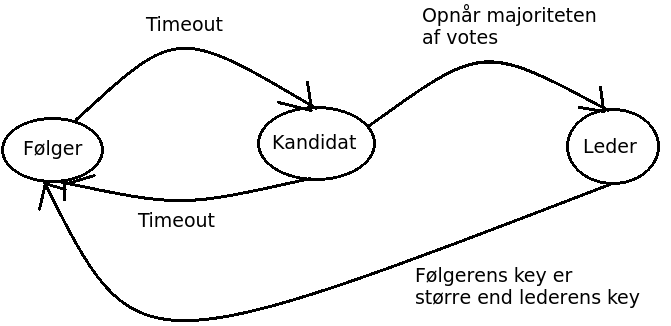
\includegraphics[width=1\textwidth]{State-machine.png}
\end{figure}
Desuden ser vi at køretiden primært er afhængig af forbindelsen og hardware til at sende data mellem maskiner. Dette betyder, at programmerings sproglige køretids-begrænsninger ikke vil have nogen reel effekt på ydeevnen af programmet. Dette har tilladt os at lave implementeringen i Python, da det tilbyder et fornuftigt socket system via standard biblioteksfunktioner.
\newpage

\section{Implementering} 
\subsection{Overordnet struktur} 

\subsubsection{Funktioner} 
Det meste af systemet foregår i klassen Heartbeat, hvorfra der laves kald til en log datastruktur designet til at fungere sammen med heartbeat klassen. Selve heartbeat klassen er opbygget af tre funktioner der beskriver systemets tilstand henholdsvis follower, candidate og leader. Disse bruges til at holde styr på hvilke opgaver der skal løses i det nuværende stadie. Disse tre funktioner håndterer alt datadeling samt leader-election og Discovery.
\\[5px]
Af disse funktioner gælder det at lederen er den der skal processere flest svar fra følgere, og kandidaten udelukkende er et midlertidig mellemstadie, der hurtigt enten skifter til leder eller følger. Dette gør at man for store systemer kan overveje, hvorvidt applikationen skal ligge lige så meget pres på lederen som på følgerne.
Disse funktioner bliver kaldt gentagne gange i en uendelig løkke for at holde programmet kørende. Dette laves endvidere i en ny tråd, således at det ikke blokerer for bruger funktionaliteterne, men samtidig bliver ved med at holde sig selv opdateret.
\\
Til sidst tilføjes bruger funktioner, der tillader brugeren, at sætte eller fjerne værdier i bruger dictionariet, samt tilgå diverse informationer fra loggen.

\subsubsection{Sammenspil mellem funktioner}
I den nuværende version af systemet sendes alt som ukrypteret klartekst via UDP som enten broadcast eller til specifikke adresser. Lederen broadcaster et heartbeat ud bestående af den nuværende logiske tid samt eventuelle log ændringer, som for eksempel “add ip-adress to list of ips”.  Disse heartbeats kan så læses af alle maskiner der er koblet til det lokale netværk og kender port nummeret bundet til broadcasten. 
\\
Såfremt disse maskiner kører heartbeat systemet, kan de svare tilbage som følgere og melde sig på listen over aktive ip adresser, samt for tildelt den delte data, herunder en liste over ip adresser, fælles bruger dictionary samt loggen over nylige ændringer. Hvis en følger viser sig at være ny eller er kommet for langt bagud, sendes der en overwrite besked, som sender alt dataen i stedet for log-opdateringer. Hvis en følger ikke modtager heartbeat broadcasts vil den efter en kort periode skifte stadie til kandidat, hvor den broadcaster og beder om stemmer, for at vide hvorvidt den kan blive den nye leder.

\subsubsection{Protokol format}
I forbindelse med implementeringen af en log i vores system, var det nødvendigt, at finde på en konkret formatering af tekst beskederne, der sendes rundt i systemet.
Denne formatering er lavet som en klartekst string der har formen:
<key><komma><Kommando><kolon><data><mellemrum><næste besked>
f.eks. bruges der i add’s tilfælde, add(1, 127.0.0.1) hvor den skal have nøglen 1: 
“1,ad:127.0.0.1”
\\
For at læse disse, og altid have en fælles længde, bruger forkortelser i stil med “se:” (set), “de:” (delete), “ad:” (add), “re:” (remove) og “co:” (commit). 


\subsection{Log}
For at strukturere den information hver maskine har om systemets stadie, samt overblik over opdateringer og de andre maskiner, er der lavet en klasse for loggen, der indeholder en liste over IP’er, en liste over opdateringer samt et bruger dictionary, som opdateres af applikationslag funktioner.
\\
Loggen bruger en parse funktion til at fortolke beskeder på protokollens format. 
Denne funktion opdaterer listerne, samt inkrementerer en key efter hver opdatering. Loggen holder endvidere styr på at rækkefølgen af kommandoer er korrekt, samt at der ikke udføres den samme kommando flere gange.
Eksempelvis ville kommandoen fra vores forrige eksempel ende med at udføre kommandoen ad(1, 127.0.0.1) efter at have været igennem parseren.
\\
Loggen består desuden af en funktion overwrite, der tillader lederen at sende alle listerne som en string, i tilfælde af at en maskine er bagud i forhold til forrige commit, der fjerner entries fra opdaterings loggen, hvis der er konsistens blandt maskinerne i systemet. Det antages, at det altid vil være gældende ved tilkobling af en ny maskine på systemet.
Såfremt en maskine kun er et par opdateringer bagud, kan man bruge funktionen compile til at skaffe de seneste opdateringer.


\subsection{Heartbeat-systemet}
Heartbeat-systemet er sådan bygget op, at alle der er en del af systemet tildeles en rolle, som enten follower, candidate eller leader. Denne rolle bestemmer efterfølgende hvilken funktion, som den enkelte klient i systemet kører.
Før der udføres noget for den konkrete rolle, så bliver der dog først sat et socket for alle de forskellige klienter, så der senere kan sendes data til/fra denne.
\\
Herudover sættes alle klienters state først og fremmest til at være follower, da der i forvejen kan være en leader aktiv, og hvis ikke, så er et leader-election nødvendigt, så den bedste leader bliver valgt.
Herefter findes og defineres alle de nødvendige variable, der senere bliver nødvendige i klassen.

\subsubsection{Leader}
Som det første tjekker vi om det er en ny leder, dette gøres ved at sikre sig at heartbeats ipList stemmer overens med loggens liste. Hvis dette gælder laver vi en ny liste af IP-adresser hvor hver ip gives en tid, hvor hvis ikke IP-adressen besvarer et heartbeat inden tiden er gået, vil adressen fjernes fra listen over aktive systemer. Denne værdi kan ændres afhængig af hvor ofte man vil heartbeate, samt størrelsen af programmet. Vi har sat den til to sekunder, hvilket svarer til at man bliver fjernet efter at have misset tre til fire heartbeats. 
Herefter sender vi et heartbeat, såfremt nuværende system tid er højere end en pågældende værdi for hvor ofte, der et heartbeat broadcastes. I heartbeatet er det første vi gør at tjekke hvorvidt det er muligt at committe de ændringer der var sket ved det forrige heartbeat. Dette gør vi ved at have en nøgle-værdi, som er den nøgle der var størst sidst vi broadcastede. Denne nøgle tjekker vi så om alle følgerne er foran. Såfremt alle følgerne svarer med en nøgle der er lig eller større end denne nøgle, så kan vi committe på nøglen.
\\
For at holde styr på hvorvidt alle i systemet er nået til enighed, og vi derved kan committe, sætter vi en variabel for antal forventede svar til længden af listen af IP-adresser, minus en grundet lederen altid er enig, hvis der er mere end en aktiv adresse. Dette gør vi grundet, at hvis der kun er lederen, så er vi ikke interesserede i at committe, da der så kun er en aktiv maskine, og derved ikke nogen maskiner at skulle være enige med.
\\[5px]
Dette antal forventede svar sætter vi så ned hver gang vi modtager en key fra en følger, som er større end den nuværende nøgle, med den antagelse at der kun kommer et svar per følger per broadcast, og at nye følgere altid sender -1, og derved aldrig er større end den nuværende nøgle.
\\
Såfremt vi ønsker at committe tilføjer vi co:currentKey, til broadcast beskeden.
Efter broadcasting, eller hvis vi ikke broadcaster denne iteration, kommer vi videre til at læse data fra følgerne. Vi tjekker første for om følgerne har sendt en set eller delete besked, fra applikationsniveauet. Disse sender vi videre til vores broadcast besked, og parser dem med lederen med det samme, for at opdatere nøglerne.
\\
Såfremt følgerne sender nøglen -1, ved vi at det er en ny følger, og vi skal derfor sende en overwrite indeholdende up-to-date log, ip liste og user dictionary. Alternativt sender vi overwrite hvis følgeren sendte en key der er mindre end lederens laveste key.
Såfremt nøglen er mindre end den nuværende nøgle, men større end laveste nøgle sender vi den manglende data via loggens compile funktion.
Herefter opdaterer vi værdierne i ip-listen. Således at hvis lederen ikke er i listen tilføjer vi den. Hvis en følger ikke har svaret tilbage inden for den givne tid, fjerner vi den fra ip-listen og loggen. Hvis følgeren svarer tilbage opdaterer vi dens levetid. 
Alle opdateringer til listen tilføjes til broadcast beskeden, så de bliver sendt ud til resten af medlemmerne i systemet.

\subsubsection{Follower}
I followeren forsøger vi at modtage data fra broadcasts, og undersøger hvad dette data indeholder.
\\
Hvis beskeden, message indeholder “Vote”, så ved vi, at der er tale om et broadcast fra en candidate, og followeren svarer derfor tilbage med “Voted” for at svare på det leader-election, som kandidaten har sat igang.
Hvis message ikke er “Vote”, så ved vi der er tale om et broadcast fra leder, og vi splitter derfor beskeden op i henholdsvis den key vi modtager, samt beskeden.
Herefter parses beskeden, via vores funktion parse.
\\
Hvis følgeren lige er kommet ind i systemet - hvilket betyder, at den har en tom log, og dens nuværende key er -1, så sender følgeren -1 tilbage til lederen, da lederen så ved, at følgeren skal have et overwrite, da følgeren ikke har den seneste log.
Hvis dette ikke er tilfældet, så svarer følgeren tilbage med sin key, så lederen ved om følgeren er up to date.
\\[5px]
Endeligt så har vi også self.timer, der hele tiden opdateres når sker nye ting, som i dette tilfælde er at modtage broadcasts fra lederen.
Hvis der går tilstrækkelig lang tid mellem, at følgeren modtager nogle beskeder fra lederen, så går den over og ændrer state til kandidat.


\subsubsection{Candidate}
I første omgang, så tæller kandidaten sig selv med, så vote-counteren sættes til 1.
Herefter broadcaster kandidaten “Vote” ud, som følgeren så modtager og behandler, som beskrevet i afsnittet om denne.
\\
Herefter sættes der en voteTimer, så det leader-election, som kandidaten sætter i gang kører for evigt.
Herefter så starter det rigtige leader-election, og det bliver kørt indtil kandidaten modtager stemmer fra mindst halvdelen af de aktive systemer, el. længden af listen over IP-adresser. Derudover så stoppes valget også, hvis vote-timeren bliver overskrevet, hvilket fører til at kandidaten går hen og bliver en følger, og vote-counteren sættes til 0.
\\
Hvis kandidaten ikke er blevet sat til følger efter valgperioden, så ved vi, at denne må have opnået nok stemmer til at blive leder, og dennes state ændres derfor.

\subsubsection{Trådning}
For at programmet kan køre og vedligeholde en liste over ip adresser, uden at blokere for brugeren, bliver programmet eksekveret i en tråd. Dette implementeres via. threading og semaphore. Dette betyder imidlertid at der er blevet taget nogle valg for at holde en konsistentet mellem heartbeat klassen og brugeren.
\\ 
Derfor er der taget nogle valg angående funktionaliteten af enkelte funktioner.
Set og delete er begge lavet ud fra at de først må returnere til når der er committed i systemet, derfor er der sat en semaphor, update event, der var på en notify all. Denne notify all bliver sendt i lederen når der sendes en commit besked, samt i følgeren når den log.parse() returnere true. Derfor er der tilføjet til funktionen parse, at den returnerer true hvis en af beskederne var en commit, og false ellers.
\\
Endvidere er der sat en lås i init, start lock, der først slippes når leaderIp er sat. Dette sikrer at brugeren ikke kan kalde set/delete før end, at der er kontakt til en leder, eller at klienten selv er leder.
\\
Dette betyder også at lederens IP-adresse skal sættes, som det første når en maskine bliver leder, til trods for at man ellers bare kunne bruge værdien myIp. 

\subsubsection{Applikations-lags funktioner}
For at kunne give brugeren mulighed for, at tilføje, fjerne og hente fra det tidligere beskrevne user-dictionary, er der lavet en række applikations-lags funktioner. \\
Fælles for disse er, at de understøtter, at en bruger kan tilføje en kommando til denne, og derudover så ventes der via den beskrevne trådning til, at kommandoen er blevet udført, el. committed på tværs af systemet, dette sikrer at funktionen ikke vil returnere førend man kan være sikker på at den værdi man har tilføjet, rent faktisk er blevet tilføjet. Alternativet ville gøre det upraktisk at programmere med.
\\[5px]
Endelig så benyttes der i alle brugerfunktionerne json-formatet \textbf{[9]}. Dette tillader os, at tilføje og hente værdier med en tilhørende key, og til fordel for vores eget format, som er beskrevet tidligere, så har vi ikke nogen begrænsninger ved, at der splittes på mellemrum eller bindestreg, og disse derved ikke kan bruges i dictionariet. Disse fordele får vi dog kun såfremt at json-formatet blev brugt over hele linjen, hvilket systemet i sin nuværende implementation mangler.
\newpage

\section{Afprøvning} 
\subsection{Runtime testning}
Til at teste, at vores Heartbeat-bibliotek virker efter hensigten, så kan vi teste systemet af på forskellige måder.
\\
Den simpleste måde er blot, at lade systemet køre og se, at der ikke undervejs opstår fejl.
Nedenfor ses en kørsel med tre maskiner, hvor der undervejs bliver til- og frakoblet en maskine af gangen. Herved kan vi se, at systemet virker under optimale forhold, samt når der undervejs opstår problemer med forbindelsen hos de individuelle maskiner. 
\\
Dette tab af forbindelse finder så blot sted, når vi dræber kørslen af programmet på den pågældende maskine.
\begin{lstlisting}
State set to: candidate
State set to: leader
Log:  []
List:  []
Log:  [[0, 'ad:192.168.43.165']]
List:  ['192.168.43.165']
Log:  [[0, 'ad:192.168.43.165'], [1, 'ad:192.168.43.49']]
List:  ['192.168.43.165', '192.168.43.49']
Log:  [[2, 'ad:192.168.43.69']]
List:  ['192.168.43.165', '192.168.43.49', '192.168.43.69']
Log:  []
List:  ['192.168.43.165', '192.168.43.49', '192.168.43.69']
Log:  [[3, 're:192.168.43.69'], [4, 're:192.168.43.49'], [5, 'ad:192.168.43.49']]
List:  ['192.168.43.165', '192.168.43.49']
Log:  []
List:  ['192.168.43.165', '192.168.43.49']
Log:  [[6, 'ad:192.168.43.69']]
List:  ['192.168.43.165', '192.168.43.49', '192.168.43.69']
Log:  []
List:  ['192.168.43.165', '192.168.43.49', '192.168.43.69']
Log:  [[7, 're:192.168.43.49']]
List:  ['192.168.43.165', '192.168.43.69']
Log:  []
List:  ['192.168.43.165', '192.168.43.69']
Log:  [[8, 're:192.168.43.69']]
List:  ['192.168.43.165']
Program slut.
\end{lstlisting}
Testresultatet er vist fra lederens synspunkt - hvilket ses af de to første linjer, hvor den pågældende maskine skifter fra at være follower, til at være kandidat, til at være leder.
\\
Herefter printes for heartbeat loggen, som viser trinvise ændringer, samt listen, ipList over nuværende aktive maskiner.
\\
Loggen viser altså, når der bliver tilføjet, ad, eller fjernet, re, en maskine fra ip-listen og ip-listen ændres herefter med den pågældende ændring.

\subsection{Prøvekørsel m. load-balancing}
Når vi har testet, at systemet uden yderligere tilføjelser virker, så kan vi gå videre og teste med nogle konkrete eksempler på, hvordan systemet kan benyttes af fremtidige brugere.
\\
Vi har her lavet et eksempel, der simulerer en styring af load-balancing. 
Til forskel fra en reel load-balancing, så har vi i dette tilfælde blot en random integer mellem 0.0 og 1.0, der skal repræsentere CPU-loaden på den pågældende maskine.
Er CPU-loaden på under 0.8, så tilføjes den konkrete maskine til listen available ips, hvilket kan bruges i et system til, at beslutte hvilke maskiner, der ikke skal tildeles opgaver.
\\
I vores tilfælde bruges denne liste dog ikke til yderligere, men viser blot at dette rent faktisk virker.
\\
Det antages yderligere i dette eksempel, at kun følgere er en del af denne load-balancing.
\begin{lstlisting}
State set to: candidate
State set to: leader
Available IPs: []
Available IPs: [u'192.168.43.69']
Available IPs: [u'192.168.43.69']
Available IPs: [u'192.168.43.69']
Available IPs: []
Available IPs: []
Available IPs: []
Available IPs: [u'192.168.43.69']
Available IPs: [u'192.168.43.165', u'192.168.43.69']  - x 9
Available IPs: [u'192.168.43.69']
Available IPs: [u'192.168.43.165', u'192.168.43.69'] - x 5
Available IPs: [u'192.168.43.69']
Available IPs: [u'192.168.43.165']
Available IPs: [u'192.168.43.165']
Available IPs: [u'192.168.43.165', u'192.168.43.69'] -  x 4
Available IPs: [u'192.168.43.69']
Available IPs: [u'192.168.43.69']
Available IPs: [u'192.168.43.69']
Available IPs: [u'192.168.43.165', u'192.168.43.69']
Program slut.
\end{lstlisting}
I denne test ses der også fra lederens synspunkt.
\\
Undervejs i testen ses det hvordan listen af tilgængelige IP-adresser opdateres, og derved kan det give et indblik i, hvordan en evt. load-balancing kan fungere i et sådant system.

\subsection{Leader-election}
For at teste leader-election kan man måle tiden, der går før, der er blevet valgt en ny leder og at en følger har opdateret, at denne er den nye leder. Dette er her gjort ved at lave et program, der tvinger lederen til at blive følger, og starter en timer i det øjeblik der skiftes til følger. Denne følger stopper så timeren ved det øjeblik at den har opdateret lederens IP-adresse til den nye leder.
\\[5px]
For at gøre dette, er der lavet en test funktion i Heartbeat modulet, der skifter staten til følger, og forhindrer denne maskine i at blive leder igen.
Dette har vi så kørt 5 gange for forskellige timeout intervaller, med en heartbeat timer på 150 ms. 
Dette giver nedenstående graf:
\\
\begin{figure}[H]
  \caption{Vores leader-election test.}
  \centering
    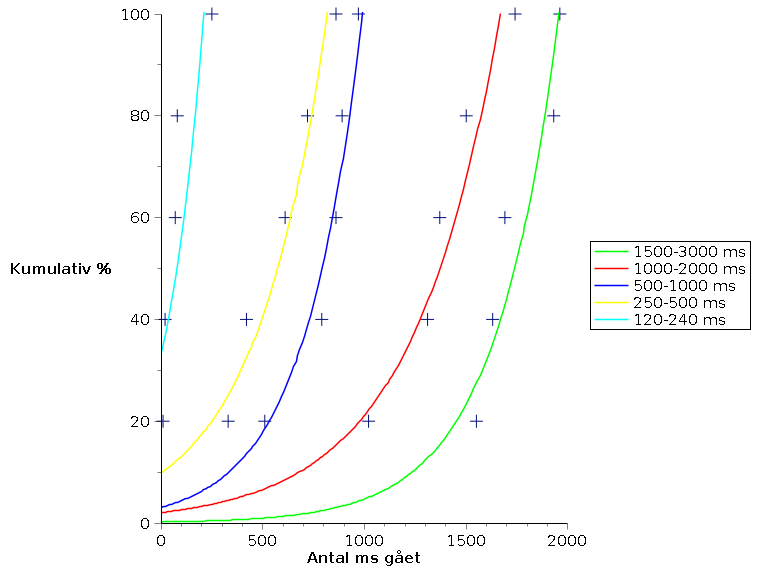
\includegraphics[width=1.2\textwidth]{Newleadergraf.png}
\end{figure}

\begin{figure}[H]
  \caption{Raft leader-election test.}
  \centering
    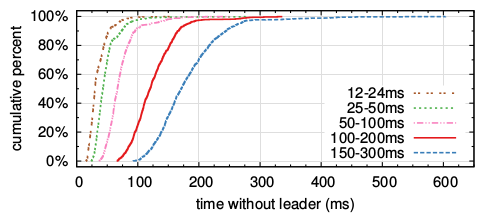
\includegraphics[width=0.8\textwidth]{Raftleadergraf.png}
\end{figure}

Grafen for vores Heartbeat system viser i stil med Raft [3], at der kommer mindre tid uden leder jo tættere man kommer på heartbeatets timer.
\\
Dog viste forsøget at jo tættere man kommer på, jo mindre tolerance er der over for missede pakker. Dette ses især i forbindelse med målingen på 120-240 ms, hvor der i de fleste tilfælde bliver valgt leder før den forrige leder er stoppet. Dette giver nogle forkerte data, da heartbeatsne fra den nye leder bliver buffet i den første leders socket, og derfor skulle den blot læse fra bufferen. Dette viser, at man nødvendigvis må være nødt til, at tage hensyn til hvor tolerant ens system skal være over for pakketab. Man kan altså ikke bare skrue helt ned for timeren uden, at det kan give problemer med systemet. 
\\
Samme kan nogenlunde ses med Rafts eksempel, hvor ca. 80-90\% allerede har valgt en leader efter få ms. Til forskel fra vores graf, så har Raft dog langt flere målinger, hvilket giver en lidt pænere kurve.

\subsection{Ydelse}
\subsubsection{Køretid}
Når man snakker om ydelse i et distribueret system som dette, vil man lægge mærke til at det er at sende beskeder som tager det meste af tiden. Dette er især gældende for heartbeat systemet da der regelmæssigt sendes beskeder.
\\
For at beregne ydelsen kan det være interessant at se på antallet af beskeder, der sendes per Heartbeat.
Som nævnt i analysen ville en alle-til-alle kobling af maskinerne kræve at der blev sendt $n^2$ beskeder per heartbeat, da alle skulle sende til alle. 
Det var da påstået at dette kunne effektiviseres ved at bruge et leder hierarki.
At dette er gældende i denne implementation kan man se ved at finde alle beskeder der bliver sendt regelmæssigt.
\\
Vi ved at der ved hvert heartbeat sendes en besked til alle maskiner, samt at alle maskiner skal svare tilbage, hvilket lederen også er afhængig af at vente på. Dette giver os 2*n beskeder. Endvidere ved vi at vi i værste tilfælde kan komme til at skulle sende en overwrite per maskine der modtager en besked. Dette giver os samlet 3*n beskeder per heartbeat.
\newpage

\subsubsection{Skalering}
Når det kommer til skalering af vores system, så er vi begrænset af, som tidligere nævnt, Maximum Transmission Unit. Denne vil vi i denne forbindelse antage ligger på 1500 \textbf{[2]}, jvf. RFC-894, bytes. Endvidere er vi nødt til at definere en standard størrelse for en string-repræsentation af en IP-adresse. Denne vil variere alt efter systemet og hvordan maskinen gemmer strings. Ved at kalde sys.getsizeof(“192.168.100.0”), har vi fået en størrelse på 34 bytes. Dette er på et 32-bit system.
\\[5px]
Ud fra disse kan man regne sig til at det maks ville være muligt at sende $1500 / 34$ eller ca. 44 IP-adresser pr. heartbeat. 
\\ 
Endvidere antager vi, at loggen altid er commitet, altså tom. Samt at user-dictionariet ikke er i brug, da vi ikke kan antage hvilken størrelse data brugeren bruger.
Da overwrite er den største besked, eftersom at den sender alle IP-adresser, ville systemet altså kunne acceptere op imod 44 brugere, fra dette skal der trækkes størrelsen af en tom liste, samt størrelsen af et tomt dictionary. Dette er samlet 168 bytes (136 for dictionary, 32 for liste). 
Dette begrænser os til maks. at have 39 aktive maskiner i systemet ad gangen, såfremt der ikke er andet data.
\\
For at kunne skalere dette, kunne man udvide programmet, så den bruger et mix af UDP og TCP. Dette ville fjerne den nuværende begrænsning på antallet af aktive maskiner i systemet, uden at miste UDP-protokollens hastighedsfordele ved mindre systemer.
\newpage

\section{Brugervejledning}
For at kunne bruge programmet, må man først initialisere heartbeat-klassen med Heartbeat(). Dette sætter et heartbeat instans i gang, der kører på en ny tråd.
\\[5px]
Når denne tråd så er sat i gang, så får klassen tildelt en state. Hvis denne state er “leader”, så ved vi med fordel, at der kun er en enkelt af maskinerne i systemet der har denne state, hvilket vil sige at det man vælger at gøre når man er leder kun sker en gang, hvorimod der i tilfældet af at staten er “follower” kan kode blive udført af flere maskiner. Dette betyder at hvis man f.eks. ønsker at sende en besked videre til klienten, ønsker man som regel kun, at sende denne besked en enkelt gang. I dette tilfælde bør det udføres fra lederen. Er man derimod interesseret i at opdatere en værdi for hver maskine med et unikt id, kan man gøre det fra follower, som set i \textbf{LoadBalancing.py} nedenstående.
Endvidere har man adgang til et fælles dictionary mellem alle maskinerne, der kan tilgås via set(key, value), delete(key) og get(key) eller ved at hente hele dictionariet via getDic.
\\
Ved set og delete gælder der, at funktionerne først vil returnere, når værdierne er sat fælles på maskinerne, så kan der foretages flere ændringer fra bruger applikationen.
\\
\lstinputlisting[language=Python]{LoadBalancing.py}
Denne instans kobler alle heartbeat-klasser på det lokale netværk sammen, og vedligeholder en liste over aktive IP-adresser, som kan tilgås via getIps.
\newpage

\section{Konklusion}
Når det kommer til den endelige, implementerede version af vores Heartbeat-biblioteket, så må det vurderes, om denne lever op til hvad der oprindeligt var formålet.
\\
Kører man biblioteket igennem, så ser man hurtigt, at nogle ting er blevet som forventet, hvor andet i større eller mindre grad har opnået det, der var hensigten bag.
\\[5px]
\textbf{Hvad er blevet opnået?}
\\
I forhold til forventningerne om at lave et bibliotek, der gør implementeringen af heartbeat systemet så nemt at bruge for brugeren som muligt, så er det her opnået, at kunne starte et heartbeat system op, blot ved at klassen.
Alt grundlæggende arbejde der udføres af heartbeatet er skjult fra brugeren, og bliver så ofte som muligt automatiseret.
\\
Endvidere ses der, at der ved overvejede timer-intervaller, som set på (figur 4), er en begrænset periode, hvor systemet ikke vil få valgt en leder.
\\
Dette er også vist i forhold til casen med load-balancing ved, at dette er blevet implementeret kort og simpelt, (se \textbf{LoadBalancing.py} fra afsnittet brugervejledning), og uden en forståelse for hvordan heartbeatet reelt fungerer.
\newpage

\section{Perspektivering}
I tilfældet af at vi stod med mere tid til projektet, så kunne man overveje, at lave følgende tilføjelser til systemet.
\\
For det første, så kunne man løse nuværende begrænsninger, ved at se på en kombination af både TCP og UDP, som ville tillade os at skifte protokol afhængig af størrelsen på systemet. Dette kunne evt. gøres ved at tjekke størrelsen af de sendte pakker og derudfra vælge protokol.
\\
Som en anden ting, kunne det vurderes om programmet skulle kunne udvides til en endnu bredere brugerskare. En måde hvorpå dette kunne gøres, var ved at lave grafisk brugerinterface til systemet, for lettere at kunne få et overblik over aktive maskiner i systemet, uden at være afhængig af en grundlæggende forståelse for programmering.
\\
For at kunne tjekke systemets reelle ydeevne, kunne det også være interessant, at prøve programmet af i større systemer, el. i den virkelige verden i eksempelvis et firma.
\newpage

\section{Litteraturhenvisninger}
\textbf{[1]} Slides fra kurset datanet - Copyright J.F Kurose and K.W. Ross, All Rights Reserved
\\[5px]
\textbf{[2]} RFC 894 - \url{https://tools.ietf.org/html/rfc894} - 1. juni 2015
\\[5px]
\textbf{[3]} Ongaro, Diego, and John Ousterhout. "In search of an understandable consensus algorithm." Proc. USENIX Annual Technical Conference. 2014.
\\[5px]
\textbf{[4]} Kermarrec, Anne-Marie, and Maarten Van Steen. "Gossiping in distributed systems." ACM SIGOPS Operating Systems Review 41.5 (2007): 2-7.
\\[5px]
\textbf{[5]} Eksempel på Bully algoritmen - \url{http://www.cs.colostate.edu/~cs551/CourseNotes/Synchronization/BullyExample.html} - 2. juni 2015
\\[5px]
\textbf{[6]} Coulouris, George F., Jean Dollimore, Tim Kindberg and Gordon Blair. Distributed systems: concepts and design. pearson education, 2012.
\\[5px]
\textbf{[7]} Kurose James, F., and W. Ross Keith. Computer Networking: A top-down approach. Sixth Edition, 2013.
\\[5px]
\textbf{[8]} Brian Vinter. Distributed Shared Memory: A Survey of Paradigms and Concepts in Distributed Shared Memory Research, May 28 1997.
\\[5px]
\textbf{[9]} Python, json dokumentation - \url{http://docs.python.org/2/library/json.html} - 7. juni 2015

\newpage


\section{Appendix}
\subsection{Heartbeat.py}
\lstinputlisting[language=Python]{Heartbeat.py}

\subsection{Log.py}
\lstinputlisting[language=Python]{Log.py}


\end{document}

